In this chapter, we propose a joint model which uses MCMC algorithm to sample boundary of phrases and 
learns distributed word vector representations and their way of composing to form phrase embeddings.
We first introduce our on-going work on learning compositional models for distributed representation for phrases. Then we present an MCMC sampling schedule which learns flexible phrase  
boundaries and jointly learn compositional models for these phrases.
\section{Introduction}
Distributed word vector representations learned from large corpora of unlabeled data have been shown to be effective in
a variety of NLP tasks, such as POS tagging~\cite{collobert2011scratch}, parsing~\cite{chen2014fast,DurrettKlein2015}, 
language modeling~\cite{bengio2003neural,mnih2007three} and machine translation~\cite{devlin-EtAl:2014:P14-1,liu-EtAl:2014:P14-1,sutskever2014sequence,kalchbrenner2013recurrent}.
These vector representations are computed using co-occurrence statistics of words and their neighboring context words.


One of the most widely used approaches to learn these vector representations is the skip-gram model described in \namecite{Mikolov:2013} and \namecite{mikolov2013distributed}. 
The skip-gram model optimizes the probability of predicting words in the context given the current center word.  
Figure~\ref{fig:skip-gram} shows a standard skip-gram structure. 


While word embeddings are usually used to compose distributed representations for larger units,
this compositionality is not used during the whole learning procedure. \namecite{socher-EtAl:2013:ACL2013} use a recursive neural network
to learn weight matrices that capture compositionality.
However, these matrices are updated using backpropagation over syntatic nodes of a parse tree and the
learning procedure is limited to the substantially 
smaller number of labeled parse trees from the Penn Treebank. The phrasal information from the large unlabeled corpus is not utilized.


In this chapter, we first introduce an extension of the skip-gram model to utilize the phrase structure in a large corpus to capture phrase compositionality and the positional information
of both words and phrases. We jointly model words in the context of words and
phrases in the context of phrases. Additionally, we enforce a compositionality constraint 
on both the input and output phrase embedding spaces which indicates how
we build the distributed vector representations for phrases from their component word vectors.
The existing framework suffers from the limitation of small lengths of phrases. We propose to use MCMC algorithms to learn flexible phrase boundaries
and jointly learn compositional models for phrase embeddings.
\section{Skip-gram model}
\label{sec:skip}
\begin{figure}
\begin{subfigure}[b]{0.4\textwidth}
        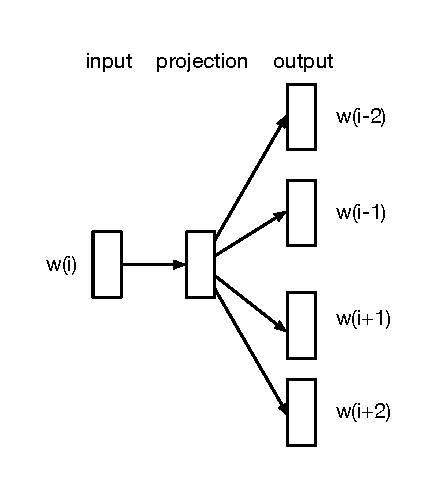
\includegraphics{./skip-gram.eps}
    \caption{word-level skip-gram}
    \label{fig:1a}
\end{subfigure}
\hfill
\begin{subfigure}[b]{0.55\textwidth}
    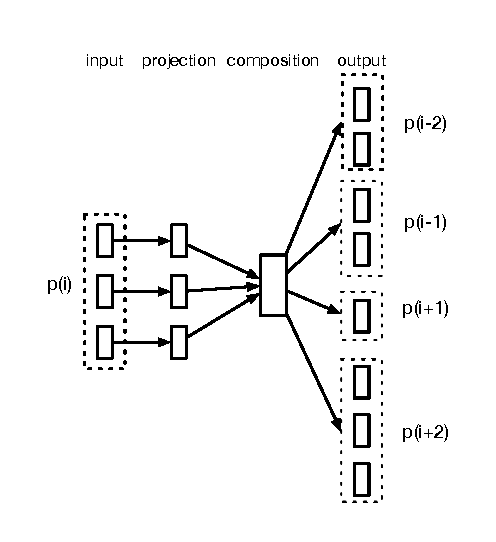
\includegraphics{./phrase-skipgram.eps}
    \caption{phrase-level skip-gram}
    \label{fig:1b}
\end{subfigure}
\caption{\small{Architecture of the skip-gram model.}}
\label{fig:skip-gram}
\vspace{-1em}
\end{figure}
The skip-gram model learns distributed vector representations for words by maximizing the probability of predicting
the context words given the current word. According to the \textit{word2vec} implementation of \namecite{mikolov2013distributed}, 
each input word $w$ is associated with a $d$-dimensional vector $v_w \in {\mathbb{R}}^{d}$ called the \textit{input embedding} and 
each context word $w_O$ is associated with a $d$-dimensional vector $v'_{w_O} \in {\mathbb{R}}^{d}$ called the \textit{output embedding}. $w, w_O$ are words from a vocabulary $V$
of size $W$. The probability of observing $w_O$ in the context of $w$ is modeled with a softmax function:
\begin{equation}
P(w_O | w) = \frac{\exp({v'_{w_O}}^T v_w)}{\sum_{i=1}^W \exp({v'_{w_i}}^T v_w)}
\end{equation}


The denominator of this function involves a summation over the whole vocabulary, which is impractical. One alternative 
to deal with the complexity issue is to sample several negative samples to avoid computing all the vocabulary. The objective
function after using negative sampling is:
\begin{equation}
    E_w = \sum_{w \in s} (\log \sigma ({v'_{w_O}}^T v_w) + \sum_{i=1}^{K} \log \sigma (-{v'_{w_i}}^T v_w))
\end{equation}
where $s$ is a chunked sentence. $w_i$, $i=1, 2, \ldots ,K$, are negative samples sampled from the following distribution:
\begin{equation}
P(w) = \frac{{\widetilde{P}(w)}^{\frac{3}{4}}}{Z}
\end{equation}
where $\widetilde{P}(w)$ is the unigram distribution of words and $Z$ is the normalization constant. The exponent $\frac{3}{4}$ is 
set empirically.
\section{Compositionality-aware skip-gram model}
\label{sec:compose}
To capture the way of composing phrase embeddings from distributed word vector representations, we extend the skip-gram model to include information from 
context of phrases and learn their compositionality from word vectors during the optimization procedure. Our phrase-level skip-gram structure is shown in
Figure~\ref{fig:1b}. 
\subsection{Phrase-level skip-gram model}
The word-level skip-gram model predicts the context words given the current word vector. Our approach further models the prediction of
context phrases given the vector representation of the current phrase vector (Figure~\ref{fig:1b}). Assume $v_p \in {\mathbb{R}}^d$ to be the $d$-dimensional 
input embedding for current phrase $p$ and $v'_{p_O}\in {\mathbb{R}}^d$ to be the output embedding for context phrase $p_O$. Using negative sampling, we model the phrase-level probability with:
\begin{equation}
\label{eq:phrase-skip}
    E_p = \sum_{p\in s} (\log \sigma ({v'_{p_O}}^T v_p) + \sum_{i=1}^{N} \log \sigma (-{v'_{p_i}}^T v_p))
\end{equation}
where $p_i$, $i= 1, 2, \ldots ,N$, are negative samples sampled according to the unigram probability of phrases raised to the same exponent $\frac{3}{4}$.


We jointly model word-level skip-gram and phrase-level skip-gram for each sentence:
\begin{equation}
E = E_w + \beta E_p
\end{equation}
where $\beta > 0$ adjusts the relative importance of the word-level and the phrase-level skipgram.
\subsection{Compositionality model}
Assume a phrase $p$ is composed of words $w_1, \ldots ,w_{n_p}$, where 
$n_p$ is the number of component words. The vector representation for $p$ is computed as:
\begin{equation}
    v_p = \Phi(\oplus( \sigma(v_{w_1}), \ldots ,\sigma(v_{w_i})))
\end{equation}
where $v_p$ is the vector representation for $p$. The function $\sigma$ is a component-wise manipulation over each dimension.
%, which can be intepreted as adjusting the dimensional values to the phrase vector space.
The symbol $\oplus$ is an operator over the component word vectors, which can be \textit{linear combination, summation, concatenation} etc. 
The mapping function $\Phi$ is a linear or non-linear manipulation over the resulting vector after the $\oplus$ operation. The same composition function is used to compute 
the output phrase embeddings $v'_{p_O}$ and $v'_{p_i}$, except that the component word vectors are $v'_{w_i}$ instead of $v_{w_i}$.


To show the effect of modeling phrase embeddings, we experiment with a composition function where $\oplus$ is \textit{linear combination} and $\Phi$ is passing the resulting matrix to the left of a weight vector $l^p = [l_1^p , l_2^p, \ldots, l_{n_p}^p]$
associated with each phrase $p$ showing how we combine the component word vectors. 
\begin{equation}
\label{eq:linear}
v_p = [\sigma(v_{w_1}), \ldots, \sigma(v_{w_{n_p}})] \begin{bmatrix} l_1^p \\ \vdots\\ l_{n_p}^p \end{bmatrix}
\end{equation}
where the function $\sigma$ is a component-wise power function over vector $v=[v_1, \ldots, v_n]$:
\begin{equation}
    \sigma(v) = [\phi(v_1), \ldots, \phi(v_n)]
\end{equation}
where $\phi(v_i)=\textit{sign}(v_i)|v_i|^{\alpha}$, $\alpha\geq 1$, is a power function over each dimension. This manipulation can be interpreted as adjusting dimensional values of word vectors to the phrase vector space.


Stochastic gradient ascent is used to update the word vectors. In equation~\ref{eq:phrase-skip}, for each word $w_j$ in $p'$, either context phrase $p_O$ or negative 
phrase sample $p_i$, the gradient is:
\begin{equation}
    \frac{\partial E_p}{\partial v'_{w_j}} = \triangledown \sigma(v'_{w_j}) (l_j^{p'} (y-\sigma({v'_{p'}}^T v_p)) v_p) 
\end{equation}
where $y=1$ for each word in $p_O$ and 0 for each word in $p_i$. $\triangledown \sigma(v'_{w_j})$ is a diagonal matrix where the $i$-th diagonal value is $\phi'({v'_{w_j}}_i)$.
For each word $w_j$ in the current phrase $p$, the gradient is:
\begin{equation}
\frac{\partial E_p}{\partial v_{w_j}} = \triangledown \sigma(v_{w_j}) (l_j^{p} ((1-\sigma({v'_{p_O}}^T v_p)) v'_{p_O} + \sum_{i=1}^{N} (-\sigma({v'_{p_i}}^T v_p)) v'_{p_i})) 
\end{equation}
\subsection{Output phrase embedding space}
Following \namecite{ling-EtAl:2015:NAACL-HLT} in 
using different output embeddings at each relative position to capture order information of context words (we call this \textit{positional} model), 
we use separate output embeddings to capture phrase-compositionality (we call this \textit{compositional} model). That is, we have a separate component 
word vector $v''$ to compose the phrase vectors in the context 
and the negative samples instead of using $v'$.
The intuition of this choice is that we don't want the compositionality information in the context or negative sample layer 
to be distorted by word-level updates. 


We further extend the phrase-level skipgram to include the order information, which
uses different output word embeddings to compose phrases at each relative position. Phrases at the same relative position share the same
output embeddings (we call this model \textit{positional+compositional}).
Without loss of generality, we experiment with the composition
described in Equation~\ref{eq:linear}. The coefficients $l_i^p$s are set to be $\frac{1}{n_p}$.
\section{Proposed methods}
\begin{table}
\centering
\begin{center}
\scalebox{0.75}{
\begin{tabular}{|l|l|l|l|l|l|l|} \hline
 length  & 1 & 2 & 3 & 4 & $\geq 5$\\ \hline
 frequency  & 525m & 137m & 62m & 22m & 15m\\ \hline
\end{tabular}}
\caption{\small{Statistics of phrase length distributions (m/million)}}
\label{tab:stats}
\end{center}
\end{table}
The phrases information are usually extracted using a chunker or based on pointwise mutual information (PMI).
For example, the phrases extracted using \textit{senna} suffer from the small average length for each phrase. We can see from 
Table~\ref{tab:stats} that most of the phrases are of length 1 and compositionality is used in very limited places.
Another problem with such kind of phrases is that the phrase boundaries are fixed and there is no way of learning compositionality
between two adjacent phrases, especially cases where different chunkings are all valid phrases. For example,
\textit{new zealand} and \textit{new zealand islanders} are both valid phrases, while \textit{senna} would chunk \textit{new zealand}
as a phrase and \textit{islanders} as a separate phrase.
\subsection{Joint MCMC sampling model}
MCMC algorithms have been used to extract phrases by iteratively going through the unlabeled data and sample from left to right, one variable at a time
at each sentence. Usually a nonparametric bayesian model based on a nonparametric prior, such as Dirichlet Process, is used to smooth the distribution of
the data and avoid overfitting. During the sampling procedure, the boundary variables would be sampled according to the posterior distribution and the phrases
in a sentence would vary whenever some of the boundary variables are flipped during the sampling procedure.


Therefore, we propose a joint MCMC sampling and compositionality learning model for phrase extraction and learning way of composing phrase embeddings. We use a log bi-linear
model to compute the probability of contexts given the phrase sequence:
\begin{equation}
P({\bf b},{\bf c}|{\bf w})= \frac{1}{Z}e^{\sum_i v'_{c_i} \cdot v_{p_i}}
\end{equation}
where ${\bf w}$ is the word sequence and ${\bf b}$ is the binary variable sequence which models the boundary information for each phrase in the sequence and ${\bf c}$ is the context sequence for the phrases in the sequence.
At each position $j$, we sample its binary value:
$$b_j \sim \frac{1}{Z} e^{\sum_i v'_{c_i} \cdot v_{p_i}}$$
where $Z$ is a constant which is agnostic to the value of $b_j$. In practice we don't have to compute all the terms in the summation as most of them are not affected by the choice $b_j$. The terms that needs to be recomputed
involves the phrases that are affected by $b_j$: $(p_1, p_2)$ when $b_j=1$ and $p_3$ when $b_j=0$. 


After we have sampled the boundary variable $b_j$ and whenever we have reached a new phrase, we use this new phrase to predict its context. This can be done using
the compositional skip-gram model we have introduced before and the vectors are updated during the procedure. As for the update, we consider a few choices for the time
of vector update: 1. whenever a binary variable is flipped. 2. whenever we have reached the end of a phrase (sampled a binary value 1). 3. update when the boundary for the whole sentence is decided.
\begin{algorithm}[t]
\small
\caption{A joint model for phrase extraction and compositionality learning}
\begin{algorithmic}[1]
\STATE{Initialize binary variables $b_1,\cdots, b_n$}
\FOR{$iter = 1,\cdots , T$:} 
    \FOR{$s = 1, \cdots, S$:}
        \FOR{$j = 1,\cdots , n$:}
            \STATE{Let $(p_1, p_2)$ be the two phrases when the $b_j=1$ and $p_3$ be the phrase when $b_j=0$}
            \STATE{Sample $b_j \sim \frac{1}{Z} e^{\sum_i v'_{c_i} \cdot v_{p_i}}$}
            \IF{$b_j = 1$}
                \STATE{Update $v_w$ for $w\in p_1$ according to the compositionality model}
            \ENDIF
        \ENDFOR
    \ENDFOR
\ENDFOR
\end{algorithmic}
\label{alg:joint}
\end{algorithm}
\subsection{Phrase independence variation}
In the previous section, we have modeled the probability of the whole sequence with a log bi-linear model. Here we consider factorizing the probability of the whole sequence into product of probility over individual phrases.
\begin{equation}
P({\bf b},{\bf c}|{\bf w}) = \prod_i P(c_i| p_i)
\end{equation}
where $P(c_i| p_i)$ is modeled with the standard skip-gram model.
\begin{equation}
P(c_i| p_i) = \prod_{p_j \in c_i} \frac{1}{Z} e^{v'_{p_j} v_{p_i}}
\end{equation}
where $Z$ is the normalization constant which sums over the whole phrase vocabulary $Q$.
\begin{equation}
Z = \sum_{p \in Q}e^{v'_p v_{p_i}}
\end{equation}
The summation over the whole vocabulary is impractical. One alternative is to use negative sampling which approximate the sum over the whole vocabulary with a few samples.
$$Z = \sum_{j} e^{v'_{p_j} v_{p_i}}$$
where $p_j$s are negative samples sampled from the same uniform distribution over phrases described in the previous sections.


We sample the binary value $b_j$ according to the following probabilities:
$$P(b_j = 1) \propto P(c_1 | p_1) \cdot P(c_2 | p_2) \cdot P(c')$$
$$P(b_j = 0) \propto P(c_3 | p_3)\cdot P(c")$$
where $P(c')$ and $P(c")$ evaluate the change of contexts for the surrounding phrases when the binary value varies.

\section{Future schedule}
I will first wrap up the compositional model learning without MCMC before the 2016 Fall. During 2016 Fall, I will partly work on using MCMC sampling to learn phrase boundaries for expand existing framework.
I will spend more time on this project after I have finished the previous two projects. Hopefully get this work done by the end of 2017 Spring. Possible target includes ACL 2017, IJCAI 2017 and EMNLP 2017.
\section{Conclusion}
In this section, we have introduced a joint model for learning phrase embeddings and phrase compositionality. To overcome the limits of the the short length of each phrase and to increase flexibility of 
phrase boundaries, we propose a joint model which uses an MCMC sampling schedule to learn flexible boundary of phrases and learns distributed phrase compositionality at the same time.
